% !TeX root = document.tex
% !TeX encoding = UTF-8 Unicode

\chapter{Controle Livre}%
\label{chapter:free-control}

\begin{mdframed}[frametitle={Atenção!}]
    A execução deste módulo se basea na existência de conexão entre o
    \textbf{Lachesis} e o \textbf{moirai}. Para parar a execução você deve
    navegar para um outro módulo. Os dados são atualizados a cada segundo mas
    apenas são aplicados quando o \textbf{moirai} os processar, o que pode levar
    mais de um tempo de amostragem, \textbf{inclusive para parar o teste}!

    \textbf{NÃO DEIXE ESTE MÓDULO EXECUTANDO SEM ESTAR POR PERTO E ATENTO!!!}
\end{mdframed}

O módulo \textit{Controle Livre} (Figura~\ref{fig:free-control}) permite
controlar a planta livremente. Nele é possível alterar os valores das saídas
manualmente nequanto o teste está em execução.

\begin{figure}[ht!]
    \centering
    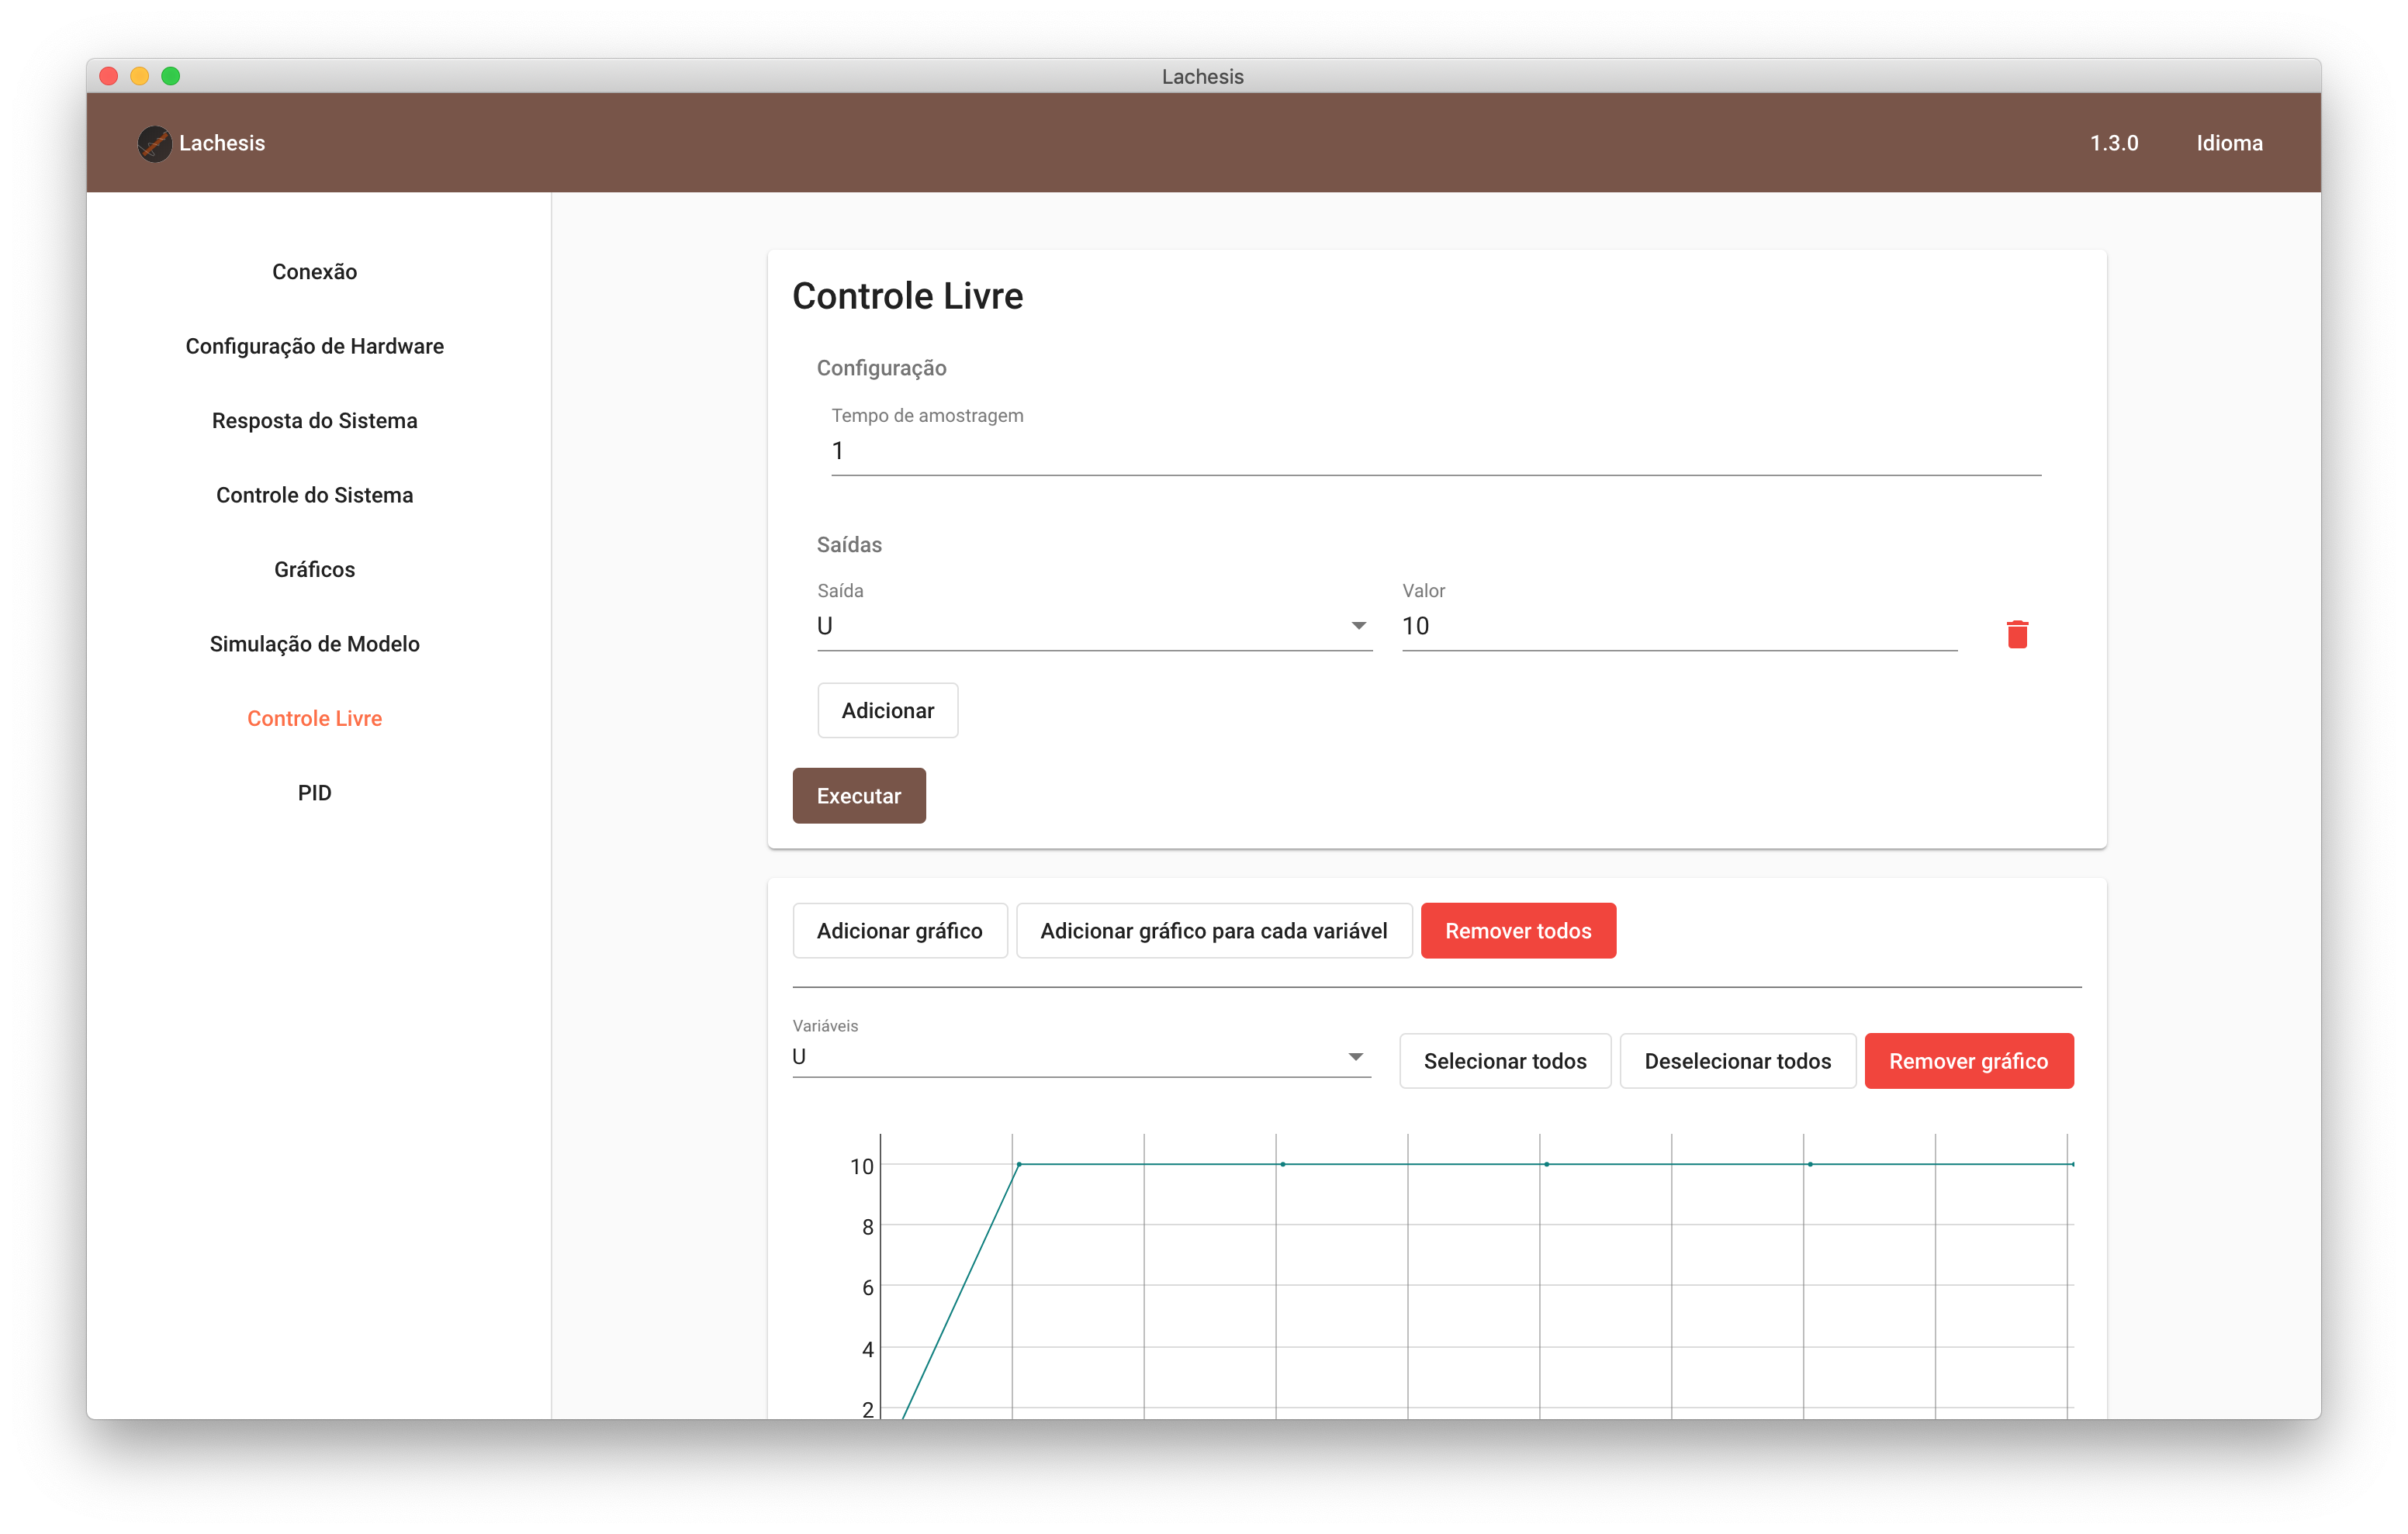
\includegraphics[width=0.9\textwidth]{imgs/free-control}
    \caption[Módulo Controle Livre]{Módulo Controle Livre}%
    \label{fig:free-control}
\end{figure}

Selecione um tempo de amostragem. É recomendado um tempo de amostragem de 1
segundo ou mais. Escolha as entradas que deseja exibir. Uma vez que o teste foi
iniciado, não é possível alterar as entradas. Adicione saídas e seus valores.
Essas podem ser modificadas enquanto o teste está em execução. Clique em
\textit{Executar}.

Com o teste em execução, os gráficos serão exibidos em uma seção ao final da
página. Todos os dados são salvos e estarão disponíveis no módulo
\textit{Gráficos}. Basta alterar o valor da saída e clicar fora do campo,
fazendo com que ele perca o foco, para que o valor seja aplicado ao sistema
real.

Pode haver uma demora de mais de um tempo de amostragem entre alterar o valor e
ele ser aplicado. Para parar o teste, basta navegar para outro módulo. É
necessário, no mínimo, um tempo de amostragem para que seja detectado a perda de
conexão e o teste seja finalizado.
